\documentclass[11pt]{article}

\usepackage{acl}
\usepackage{times}
\usepackage{latexsym}
\usepackage{booktabs}
\usepackage{multirow}
\usepackage[T1]{fontenc}
\usepackage[utf8]{inputenc}
\usepackage{microtype}
\usepackage{inconsolata}
\usepackage{graphicx}
\usepackage{tikz}
\usetikzlibrary{shapes.geometric, arrows.meta, positioning, fit, backgrounds}

\title{Semantic Decomposition of Software Requirements Using Large Language Models}

\author{Ali Edrisabadi, \ {\bf Sahand Seyed Mohammadghavami,} \ {\bf Amirhesam Torkashvand} \\ {\bf Amirhossein Shirvani Dastgerdi,} \ {\bf Sabra Hashmebeigi} 
          \\ {\ Politecnico di Torino}}

\begin{document}
\maketitle

\begin{abstract}
Natural language software requirements frequently suffer from ambiguity, inconsistency, and incompleteness, leading to defects in later development stages. While large language models (LLMs) offer promising capabilities for requirements analysis, their direct application often produces inconsistent outputs without structural guidance. This study investigates whether LLMs can reliably decompose requirements into semantic abstractions---including actors, actions, conditions, and system responses---and compares single-step baseline tagging against a multi-step pipeline approach. Evaluation on 50 requirements from a library room booking system reveals that single-step baseline tagging achieves the best performance (Micro-F1=0.65 with zero-shot prompting), while the more complex pipeline approach underperforms. Our results suggest that simpler prompting strategies may be more effective for semantic annotation tasks with current LLM capabilities.
\end{abstract}

\section{Introduction}

The evolution toward complex software systems has been accompanied by growth in the volume and intricacy of engineering requirements \citep{Norheim2024}. These requirements are predominantly expressed in natural language, necessitating substantial human expertise for elicitation, documentation, and management \citep{Zhao2022}.

Many defects and cost overruns in software development can be traced to issues in requirements engineering \citep{Aurum2005}. Among the most cited challenges are ambiguity, inconsistency, and incompleteness \citep{Femmer2017, Zhao2022}, which lead to misinterpretation, overlooked constraints, or conflicting specifications.

Natural language processing (NLP) techniques have long been viewed as promising for requirements engineering, yet earlier approaches failed to deliver scalable benefits \citep{Berry2012}. The advent of large language models (LLMs) has sparked renewed enthusiasm, with expectations that their semantic understanding might overcome historical limitations \citep{Norheim2024}.

However, direct application of LLMs remains fraught with risks, including hallucination and failure to capture nuanced domain intent \citep{Norheim2024}. We investigate structured approaches based on semantic decomposition into explicitly defined abstraction layers.

\subsection{Research Questions}
\begin{itemize}
    \item \textbf{RQ1:} Can LLMs reliably identify semantic abstractions (e.g., \textit{Main\_actor}, \textit{System\_response}, \textit{Condition}) within requirement text?
    \item \textbf{RQ2:} Does a multi-step decomposition pipeline improve annotation quality compared to single-step tagging?
    \item \textbf{RQ3:} How do different prompting strategies (zero-shot, one-shot, few-shot) affect performance?
\end{itemize}

\section{Related Work}

Requirements engineering emphasizes clarity, testability, and consistency, but achieving these properties is difficult with free-form natural language. Prior approaches include controlled natural languages and templates such as EARS \citep{Mavin2009, Rupp2014}.

Writing effective requirements is central to successful systems engineering \citep{Hull2005}. Requirements can be expressed in textual or graphical forms \citep{Bruel2021}, ranging from informal natural language to formal specifications. However, most real-world requirements remain in unconstrained natural language \citep{Zhao2022}.

NLP has long been viewed as promising for automating RE \citep{Ryan1993}. Early efforts focused on rule-based techniques \citep{Kof2005}, while recent machine-learning approaches improved ambiguity detection and classification \citep{Zhao2022, Sonbol2022}. Transformer-based LLMs have shifted the landscape \citep{Vaswani2017}, demonstrating remarkable zero-shot and few-shot capabilities \citep{Brown2020}. In RE, LLMs show promise for generation, quality assessment, and classification \citep{Norheim2024}. Structured decomposition approaches, drawing on goal-oriented methodologies such as KAOS \citep{vanLamsweerde2000} and i* \citep{Yu1997}, represent a relevant direction.

\section{Methodology}

\subsection{Semantic Abstraction Schema}

We define eight semantic tags capturing key building blocks of requirements:

\begin{itemize}
  \item \textbf{Main\_actor}: Primary actor initiating or benefiting from the requirement.
  \item \textbf{Entity}: Noun phrases and objects (UI elements, data items, resources).
  \item \textbf{Action}: What the actor does or intends (verb phrases).
  \item \textbf{System\_response}: What the system shall do (outputs, state changes).
  \item \textbf{Condition}: If/when/while clauses constraining behavior.
  \item \textbf{Precondition}: State that must hold before the requirement applies.
  \item \textbf{Constraint}: Quantitative or qualitative limits (time, format, performance).
  \item \textbf{Exception}: Unless/except/otherwise clauses for edge cases.
\end{itemize}

\begin{figure}[t]
  \centering
  \includegraphics[width=0.95\columnwidth]{Capture.PNG}
  \caption{Example of semantically annotated requirements showing identified abstractions.}
  \label{fig:example}
\end{figure}

\subsection{System Architecture}

Figure~\ref{fig:architecture} illustrates our two approaches for semantic decomposition.

\begin{figure}[t]
\centering
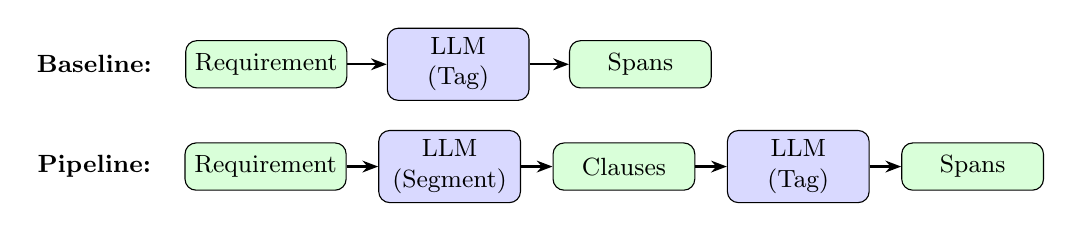
\begin{tikzpicture}[
    node distance=0.4cm and 0.6cm,
    box/.style={rectangle, draw, rounded corners, minimum width=1.8cm, minimum height=0.6cm, align=center, font=\small},
    llmbox/.style={box, fill=blue!15},
    databox/.style={box, fill=green!15},
    arrow/.style={-{Stealth[length=2mm]}, thick}
]

\node[font=\small\bfseries] (baseline_label) {Baseline:};
\node[databox, right=0.3cm of baseline_label] (req1) {Requirement};
\node[llmbox, right=0.5cm of req1] (llm1) {LLM\\(Tag)};
\node[databox, right=0.5cm of llm1] (spans1) {Spans};

\draw[arrow] (req1) -- (llm1);
\draw[arrow] (llm1) -- (spans1);

\node[font=\small\bfseries, below=0.8cm of baseline_label] (pipeline_label) {Pipeline:};
\node[databox, right=0.3cm of pipeline_label] (req2) {Requirement};
\node[llmbox, right=0.4cm of req2] (llm2a) {LLM\\(Segment)};
\node[databox, right=0.4cm of llm2a] (clauses) {Clauses};
\node[llmbox, right=0.4cm of clauses] (llm2b) {LLM\\(Tag)};
\node[databox, right=0.4cm of llm2b] (spans2) {Spans};

\draw[arrow] (req2) -- (llm2a);
\draw[arrow] (llm2a) -- (clauses);
\draw[arrow] (clauses) -- (llm2b);
\draw[arrow] (llm2b) -- (spans2);

\end{tikzpicture}
\caption{Architecture comparison: Baseline (single-step) vs. Pipeline (two-step with segmentation).}
\label{fig:architecture}
\end{figure}

\paragraph{Baseline Approach}
A single LLM prompt directly annotates the full requirement with semantic spans in one pass, outputting structured JSON.

\paragraph{Pipeline Approach}
The task is decomposed into two stages: (1) \textbf{Segmentation} splits the requirement into logically coherent clauses; (2) \textbf{Tagging} annotates each segment with semantic abstractions.

\paragraph{Implementation}
All experiments use Qwen3 4B via the Ollama framework. Temperature is set to 0.2 for reproducibility. We test three prompting strategies: zero-shot, one-shot, and few-shot (3 examples).

\subsection{Dataset}

The evaluation dataset consists of 50 requirements from an online library study room booking system. Table~\ref{tab:dataset} shows the distribution by complexity.

\begin{table}[t]
\centering
\small
\begin{tabular}{lcc}
\toprule
\textbf{Complexity} & \textbf{Count} & \textbf{Example Pattern} \\
\midrule
Simple & 23 & ``The system shall display X'' \\
Conditional & 16 & ``If X, the system shall Y'' \\
Nested & 11 & Multiple conditions/exceptions \\
\midrule
\textbf{Total} & \textbf{50} & \\
\bottomrule
\end{tabular}
\caption{Dataset distribution by requirement complexity.}
\label{tab:dataset}
\end{table}

A human-annotated gold standard was constructed with span boundaries and semantic labels, enabling both exact and relaxed matching.

\subsection{Evaluation Metrics}

We evaluate using span-level Precision (P), Recall (R), and F1 with relaxed matching: spans matched using IoU for position overlap and text similarity ($score = 0.65 \times IoU + 0.35 \times TextSim$, threshold $\geq 0.5$).

\section{Results}

Tables~\ref{tab:zero}, \ref{tab:one}, and \ref{tab:few} present per-tag results for each prompting strategy.

\begin{table}[t]
\centering
\small
\begin{tabular}{lcccccc}
\toprule
& \multicolumn{3}{c}{\textbf{Baseline}} & \multicolumn{3}{c}{\textbf{Pipeline}} \\
\cmidrule(lr){2-4} \cmidrule(lr){5-7}
\textbf{Tag} & P & R & F1 & P & R & F1 \\
\midrule
Main\_actor & .84 & .82 & .83 & .29 & .33 & .31 \\
Entity & .60 & .65 & .63 & .58 & .35 & .44 \\
Action & .43 & .77 & .55 & .24 & .46 & .32 \\
System\_resp. & .74 & .93 & .82 & .47 & .33 & .39 \\
Condition & .56 & .96 & .71 & .46 & .88 & .60 \\
Precondition & .00 & .00 & .00 & .20 & .25 & .22 \\
Constraint & .58 & .23 & .33 & .86 & .20 & .32 \\
Exception & 1.0 & .50 & .67 & 1.0 & .50 & .67 \\
\midrule
\textbf{Micro-F1} & \multicolumn{3}{c}{\textbf{0.65}} & \multicolumn{3}{c}{0.40} \\
\textbf{Macro-F1} & \multicolumn{3}{c}{0.57} & \multicolumn{3}{c}{0.41} \\
\bottomrule
\end{tabular}
\caption{Zero-shot results (relaxed matching, threshold=0.5).}
\label{tab:zero}
\end{table}

\begin{table}[t]
\centering
\small
\begin{tabular}{lcccccc}
\toprule
& \multicolumn{3}{c}{\textbf{Baseline}} & \multicolumn{3}{c}{\textbf{Pipeline}} \\
\cmidrule(lr){2-4} \cmidrule(lr){5-7}
\textbf{Tag} & P & R & F1 & P & R & F1 \\
\midrule
Main\_actor & .58 & .85 & .69 & .43 & .69 & .53 \\
Entity & .32 & .81 & .46 & .35 & .83 & .49 \\
Action & .32 & .60 & .42 & .25 & .66 & .37 \\
System\_resp. & .31 & .67 & .42 & .21 & .11 & .15 \\
Condition & .43 & .92 & .59 & .40 & .88 & .55 \\
Precondition & .00 & .00 & .00 & .00 & .00 & .00 \\
Constraint & .67 & .47 & .55 & .68 & .43 & .53 \\
Exception & .00 & .00 & .00 & .50 & .50 & .50 \\
\midrule
\textbf{Micro-F1} & \multicolumn{3}{c}{\textbf{0.50}} & \multicolumn{3}{c}{0.46} \\
\textbf{Macro-F1} & \multicolumn{3}{c}{0.39} & \multicolumn{3}{c}{0.39} \\
\bottomrule
\end{tabular}
\caption{One-shot results (relaxed matching, threshold=0.5).}
\label{tab:one}
\end{table}

\begin{table}[t]
\centering
\small
\begin{tabular}{lcccccc}
\toprule
& \multicolumn{3}{c}{\textbf{Baseline}} & \multicolumn{3}{c}{\textbf{Pipeline}} \\
\cmidrule(lr){2-4} \cmidrule(lr){5-7}
\textbf{Tag} & P & R & F1 & P & R & F1 \\
\midrule
Main\_actor & .60 & .95 & .73 & .47 & .85 & .61 \\
Entity & .32 & .79 & .45 & .34 & .79 & .48 \\
Action & .34 & .60 & .43 & .30 & .51 & .38 \\
System\_resp. & .31 & .59 & .41 & .33 & .52 & .40 \\
Condition & .43 & .96 & .59 & .44 & .92 & .60 \\
Precondition & .00 & .00 & .00 & .00 & .00 & .00 \\
Constraint & .56 & .50 & .53 & .60 & .30 & .40 \\
Exception & .50 & .50 & .50 & .50 & .50 & .50 \\
\midrule
\textbf{Micro-F1} & \multicolumn{3}{c}{\textbf{0.51}} & \multicolumn{3}{c}{0.48} \\
\textbf{Macro-F1} & \multicolumn{3}{c}{0.46} & \multicolumn{3}{c}{0.42} \\
\bottomrule
\end{tabular}
\caption{Few-shot results (relaxed matching, threshold=0.5).}
\label{tab:few}
\end{table}

\subsection{RQ1: Abstraction Identification}

The LLM demonstrates varying capability across tag types. High-frequency tags with clear linguistic markers achieve strong results: \textit{Main\_actor} (F1=0.83), \textit{System\_response} (F1=0.82), and \textit{Condition} (F1=0.71) in zero-shot baseline. However, \textit{Precondition} consistently fails (F1=0.00 in most configurations), likely due to its semantic overlap with \textit{Condition} and rarity in the dataset (only 4 gold instances).

\subsection{RQ2: Baseline vs. Pipeline}

Contrary to our initial hypothesis, the \textbf{Baseline approach consistently outperforms Pipeline} across all prompting strategies:
\begin{itemize}
    \item Zero-shot: Baseline 0.65 vs. Pipeline 0.40 (+25 points)
    \item One-shot: Baseline 0.50 vs. Pipeline 0.46 (+4 points)
    \item Few-shot: Baseline 0.51 vs. Pipeline 0.48 (+3 points)
\end{itemize}

The pipeline's two-stage approach introduces error propagation: segmentation errors cascade into tagging errors. The intermediate clause representation also loses global context that helps identify cross-clause relationships.

\subsection{RQ3: Prompting Strategy Impact}

Counter-intuitively, \textbf{zero-shot prompting achieves the best results} (Micro-F1=0.65), outperforming both one-shot (0.50) and few-shot (0.51). This suggests that for the Qwen3 4B model, few-shot examples may introduce noise or bias the model toward example-specific patterns rather than generalizing to the full tag schema.

\section{Discussion}

\paragraph{Why Baseline Outperforms Pipeline}
The pipeline approach was designed to handle complex, multi-clause requirements by isolating segments. However, this decomposition: (1) introduces segmentation errors that propagate; (2) removes global context needed to distinguish similar tags; (3) doubles the number of LLM calls, increasing variance.

\paragraph{Why Zero-shot Works Best}
Zero-shot prompting allows the model to rely on its pre-trained understanding of the tag definitions without being biased by potentially non-representative examples. The model's internal priors may align better with the task than the specific patterns shown in examples.

\paragraph{Limitations}
This study is limited by: (1) single domain evaluation; (2) one model family (Qwen3 4B); (3) small dataset (50 requirements). The \textit{Precondition} tag's consistent failure suggests the tag schema may need refinement.

\section{Conclusion}

This study compared baseline and pipeline approaches for LLM-based semantic annotation of requirements. Contrary to expectations, the simpler single-step baseline consistently outperformed the two-step pipeline, with zero-shot prompting achieving the best Micro-F1 of 0.65.

Key findings: (1) Complex multi-step workflows do not necessarily improve LLM performance---simpler approaches may be more robust; (2) Zero-shot prompting can outperform few-shot for well-defined tasks; (3) Tag schema design critically impacts performance, as seen with \textit{Precondition}'s consistent failure.

Future work will explore: (1) larger models where pipeline benefits may emerge; (2) refined tag schemas with clearer distinctions; (3) hybrid approaches combining baseline simplicity with targeted pipeline use for specific complex cases.

\bibliography{custom}

\end{document}
